\documentclass[10pt]{beamer}
\usepackage{lmodern}
%\usetheme{Darmstadt}
\usetheme{Frankfurt}
\usepackage{tcolorbox}
%\usepackage{beamerthemesplit}
\usepackage{appendixnumberbeamer}
\usefonttheme{serif}
\useinnertheme{circles}
\setbeamertemplate{footline}[page number]{}
\setbeamertemplate{navigation symbols}{}
\setbeamercolor{block title}{bg=blue!30,fg=black}
%\usepackage[timeinterval=10,timeduration=2.0]{tdclock}
\usepackage{tikz}
\usepackage{graphicx}
\usepackage{subfig}
\usepackage{latexsym,amsmath,amssymb}
\usepackage{multirow}
\usepackage{amsthm}
\usepackage{epstopdf}
\usepackage{booktabs}
\usepackage{mathrsfs}
\usepackage{boldline}
\usepackage{tabularx}
\usepackage{stackengine}
\usetikzlibrary{arrows,shapes,calc}

%\usepackage[inline]{enumitem}
\usepackage{caption}
%\usepackage{subcaption}
\newcommand{\R}{{\mathbb R}}
\newcommand{\C}{{\mathbb C}}
\newcommand{\sign}{\mathop{\bf sign}}
\newcommand{\N}{\mathcal{N}}
\newcommand{\argmin}{\mathop{\rm argmin}}
\newcommand{\etc}{{\it etc.}}
\newcommand{\eg}{{\it e.g.}}
\newtheorem{proposition}[theorem]{Proposition}


%From CI paper
\let\oldcite=\cite                                                              
\renewcommand{\cite}[1]{\textcolor[rgb]{0.2,0.5,.3}{\oldcite{#1}}}
\definecolor{mycite}{rgb}{0.4,0.0,0.8}
\definecolor{myhighlight1}{rgb}{0.758, 0.2, 0.078}
\definecolor{mycite2}{rgb}{0.2,0.5,.3}


\newcommand\blfootnote[1]{%
  \begingroup
  \renewcommand\thefootnote{}\footnote{#1}%
  \addtocounter{footnote}{-1}%
  \endgroup
}
\graphicspath{ {Img/} }
\AtBeginSection[]{
	\begin{frame}{Outline}
		\tableofcontents[currentsection]
	\end{frame}
	}
\title[Deep Learning]{Introduction to Deep Learning in Vision: Basics, Optimization,  Networks and Coding}
\author[Yue Zhang]{Yue Zhang}
\institute[CWRU] {\footnotesize{Department of Mathematics, Applied Mathematics and Statistics\\ Case Western Reserve University}\\~ \\ \date \\}

\begin{document}

\begin{frame}
\titlepage
%\initclock
\end{frame}


\section{Overview}
\begin{frame}
\frametitle{Overview of the Journey}
	\begin{figure}[H]
		\centerline{
			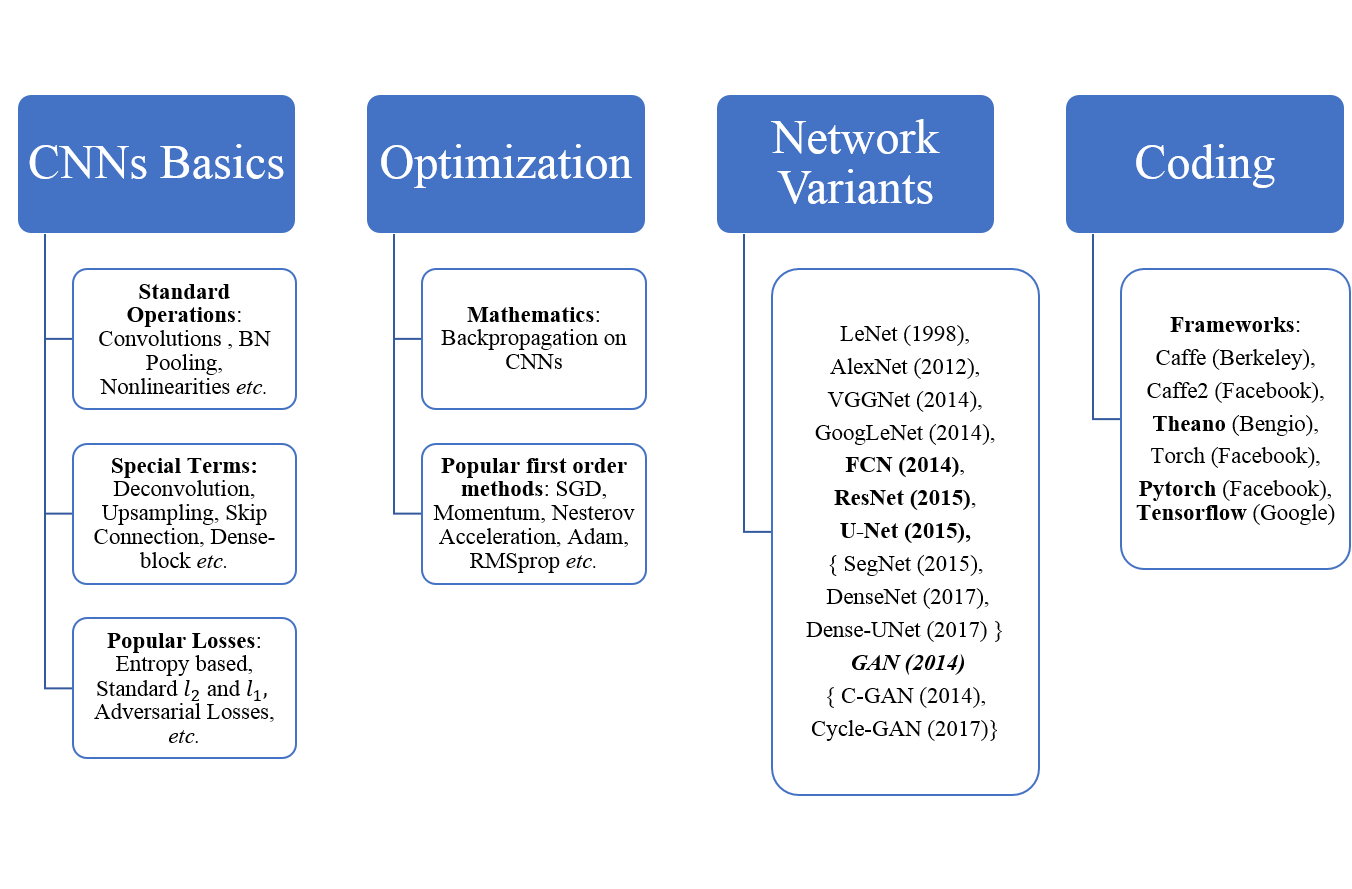
\includegraphics[width=1.1\textwidth]{overview.png}
		}
	\end{figure}
\end{frame}


\section{Convolutional Neural Networks Basics}
\subsection{Basic Operations}
\begin{frame}
	\frametitle{Basic Operations in  CNNs}
	Standard operations in a Convolutional Neural Network:
	\begin{itemize}
		\item Convolution
		\item Pooling 
		\item Batch Normalization
		\item Nonlinear Activation
		\item Others: Deconvolution, Upsampling,  Skip Connections \etc
	\end{itemize}
\end{frame}

\begin{frame}
	\frametitle{A Quick Example: UNet \blfootnote{\textcolor{mycite2}{Olaf Ronneberger, Philipp Fischer, Thomas Brox}.\textit{ U-Net: Convolutional Networks for Biomedical
			Image Segmentation}, MICCAI 2015.}}
	One of the most popular networks in semantic segmentation.
	\begin{figure}[H]
	\centerline{
		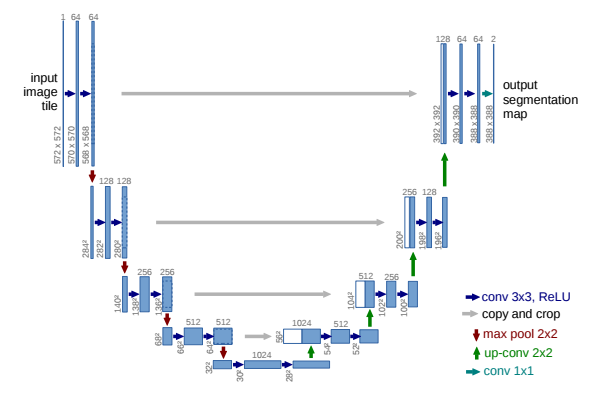
\includegraphics[width=0.8\textwidth]{unet.png}
	}
	\end{figure}
\end{frame}

\begin{frame}
	\frametitle{A Quick Example: UNet \blfootnote{\textcolor{mycite2}{Olaf Ronneberger, Philipp Fischer, Thomas Brox}.\textit{ U-Net: Convolutional Networks for Biomedical
			Image Segmentation}, MICCAI 2015.}}
		One of the most popular networks in semantic segmentation.
	\begin{figure}[H]
		\centerline{
			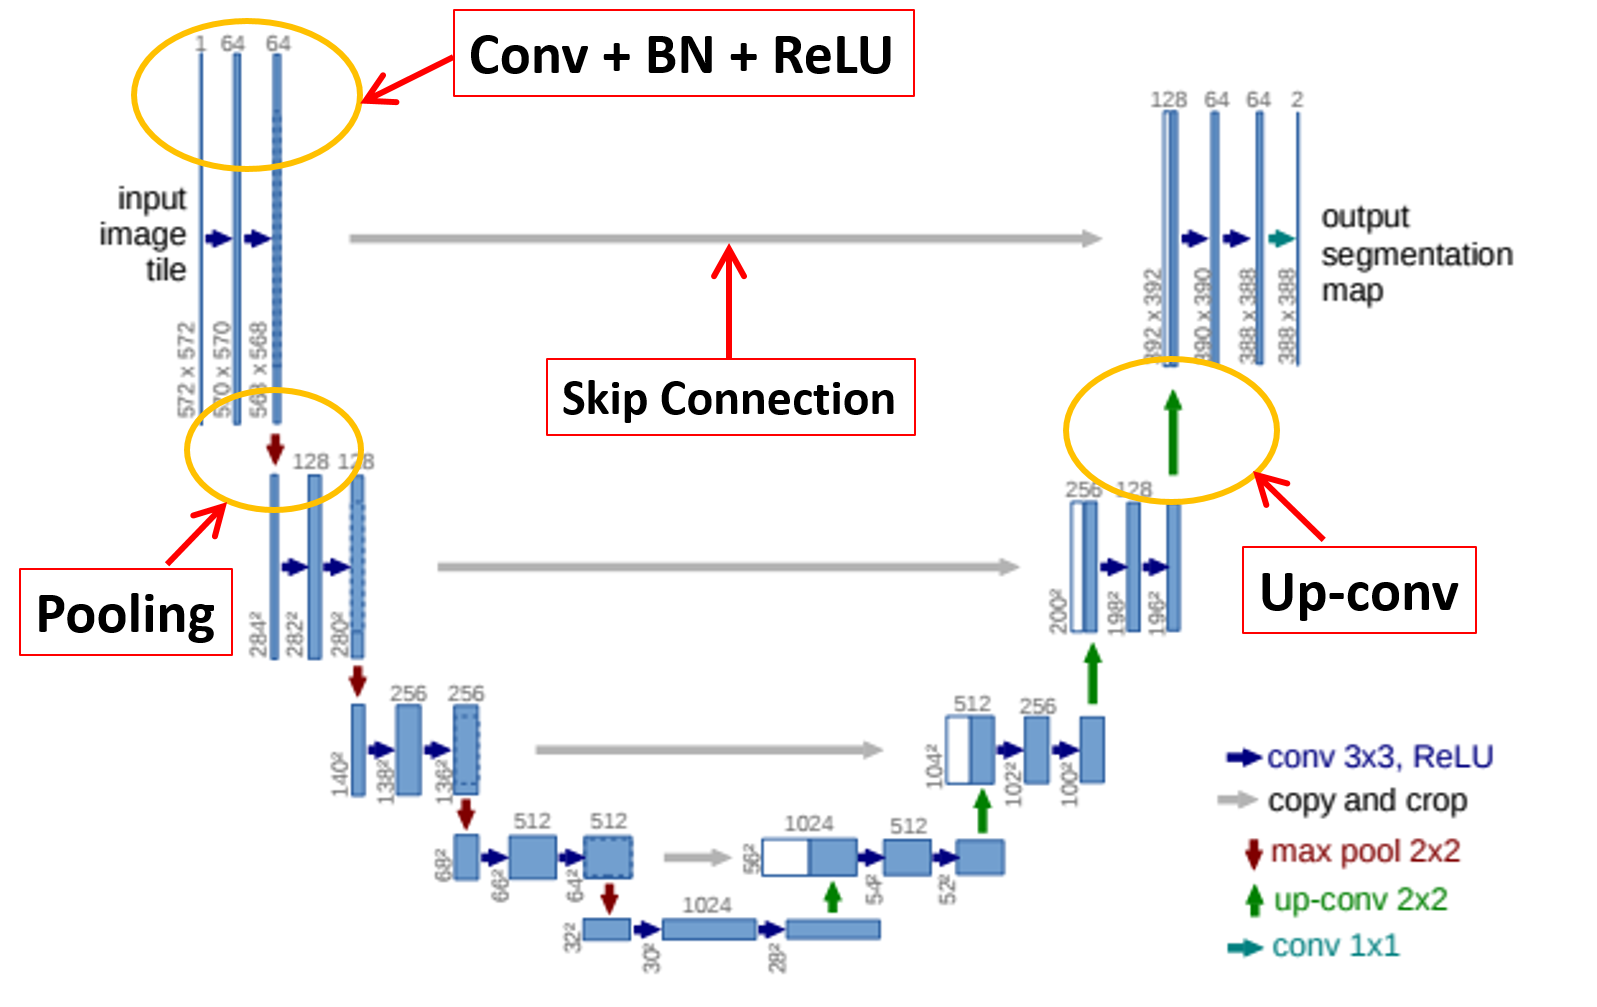
\includegraphics[width=0.8\textwidth]{unet_detailed.png}
		}
	\end{figure}
\end{frame}

\begin{frame}
	\frametitle{Convolution and Convolution Layer \\(\textcolor{pink}{\textbf{Conv}} + BN + ReLU)}
	\textit{Keywords} in Convolution: $\bullet$ \textbf{Kernel Size} \quad $\bullet$ \textbf{Stride} \quad $\bullet$ \textbf{Padding} 
	\begin{figure}[H]
	\centerline{
		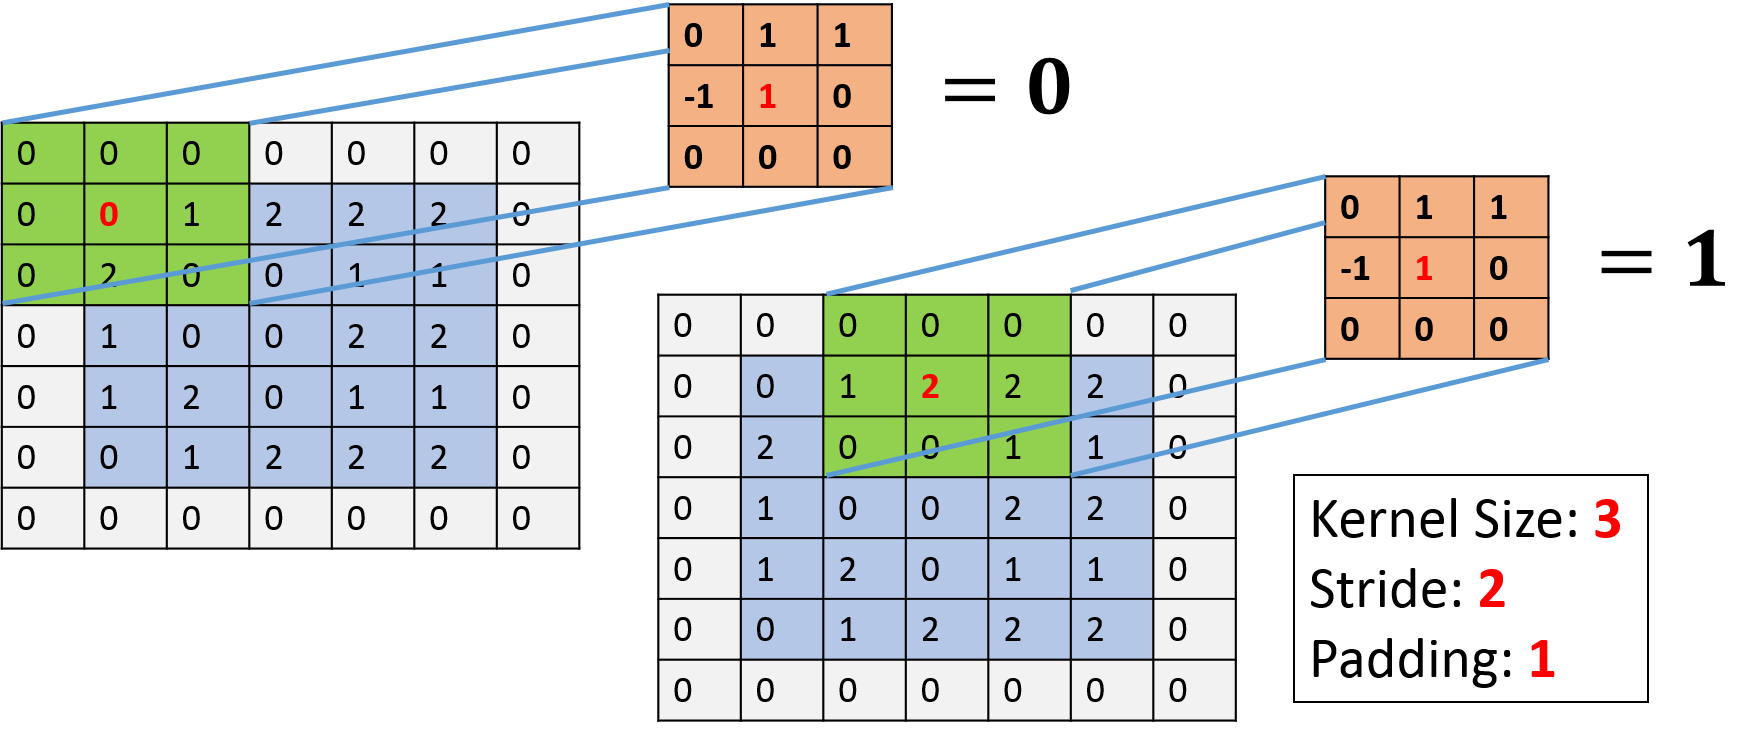
\includegraphics[width=1.0\textwidth]{convolution.png}
	}
	\caption{Illustration of Convolution\footnote{To make it simple, the kernel is already \textbf{rotated}. Only point-wise product and summation is needed}.}
	\end{figure}	
\end{frame}

\begin{frame}
	\frametitle{Convolutions in CNNs: (\textcolor{pink}{\textbf{Conv}} + BN + ReLU)}
	Different types of convolutions. 
	\begin{itemize}
		\item \textbf{Convolution}: (with/without) padding, (1/$>1$) stride.
		\item \textbf{Transposed  Convolution (Deconvolution)}: (with/without) padding, (1/$>1$) stride.
		\item \textbf{Dilated Convolution}.
	\end{itemize}
	\vskip 0.2in
	See the attached HTML file. 
	\vskip 0.2in
	Helpful reading: \textcolor{mycite2}{Vincent Dumoulin, Francesco Visin.} \textit{A guide to convolution arithmetic for deep learning. }
\end{frame}

\begin{frame}
	\frametitle{Convolutional Layer (1st): (\textcolor{pink}{\textbf{Conv}} + BN + ReLU)}
	\begin{figure}[H]
	\centerline{
		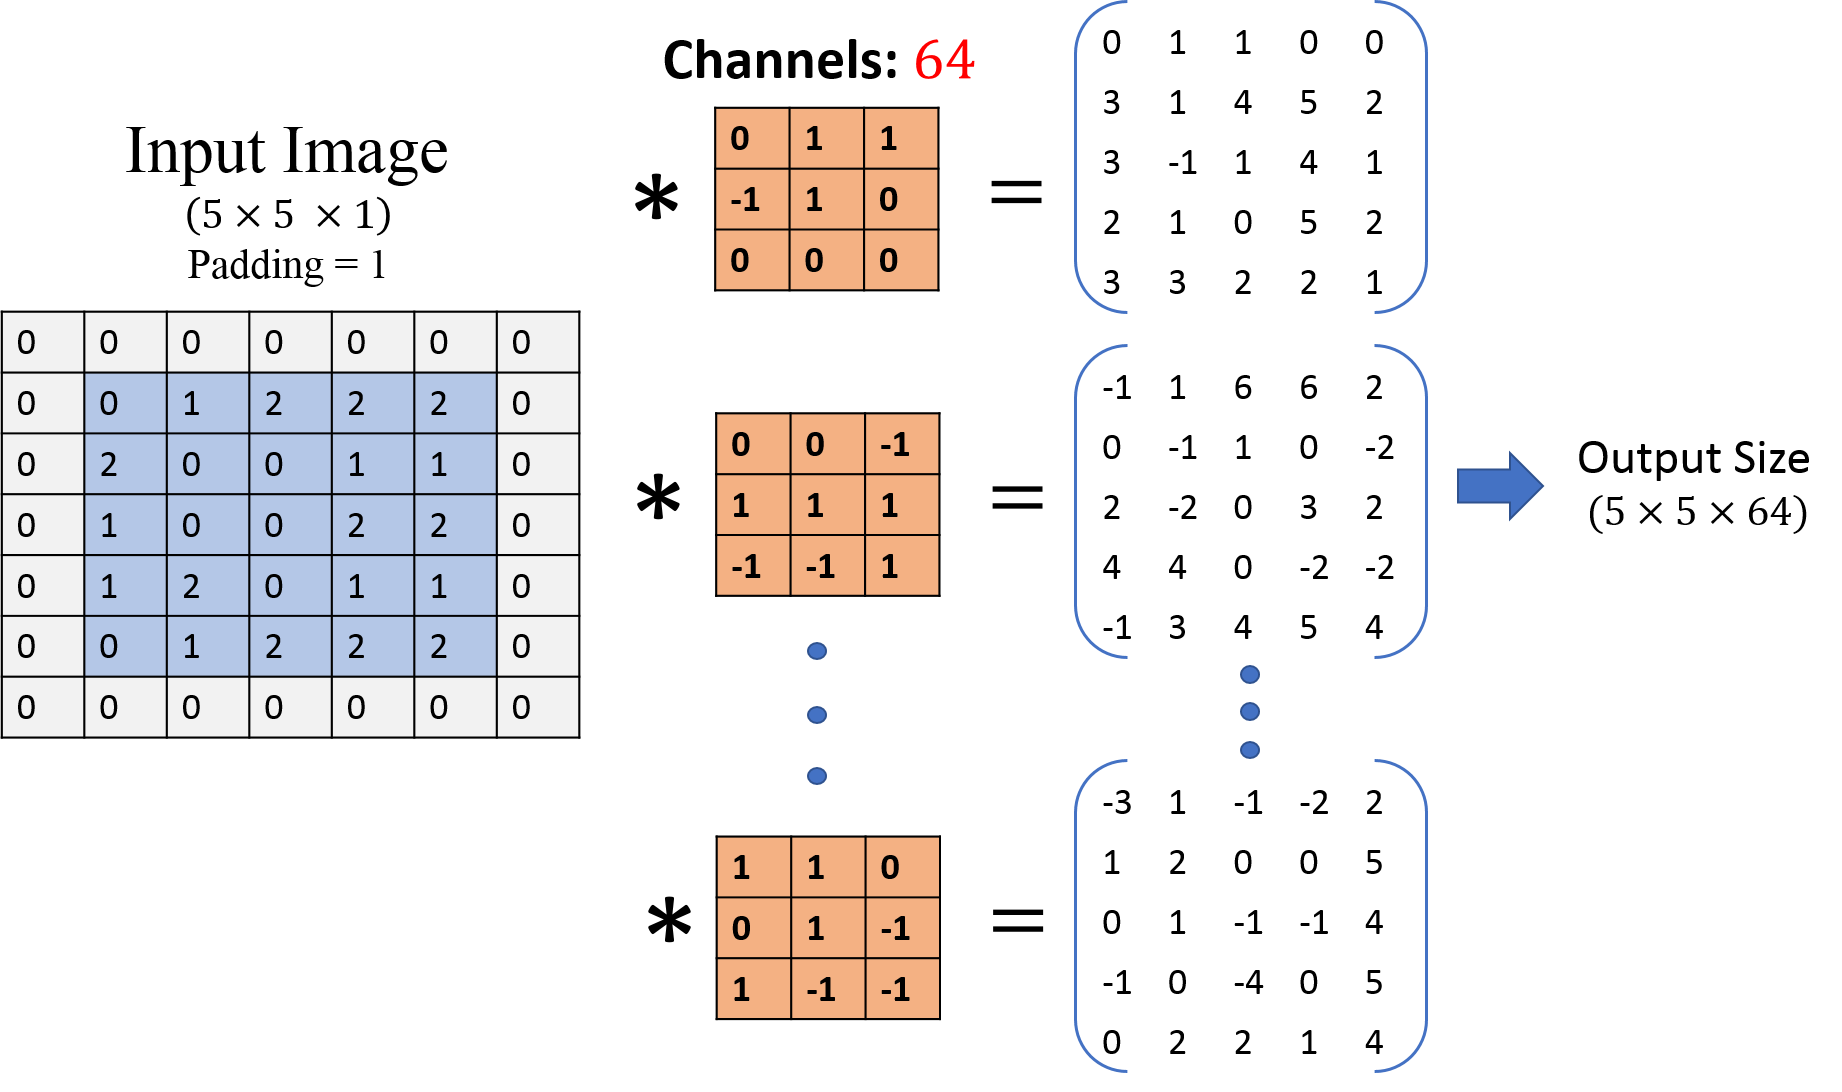
\includegraphics[width=1.0\textwidth]{convolution_1st_layer.png}
	}
	\caption{First Layer of CNN\footnote{Again, all the kernels are already \textbf{rotated}. Only point-wise product and summation is needed.}.}
	\end{figure}		
\vskip -0.2in
\end{frame}

\begin{frame}
\frametitle{Convolutional Layer (2nd): (\textcolor{pink}{\textbf{Conv}} + BN + ReLU)}
	\begin{figure}[H]
		\centerline{
			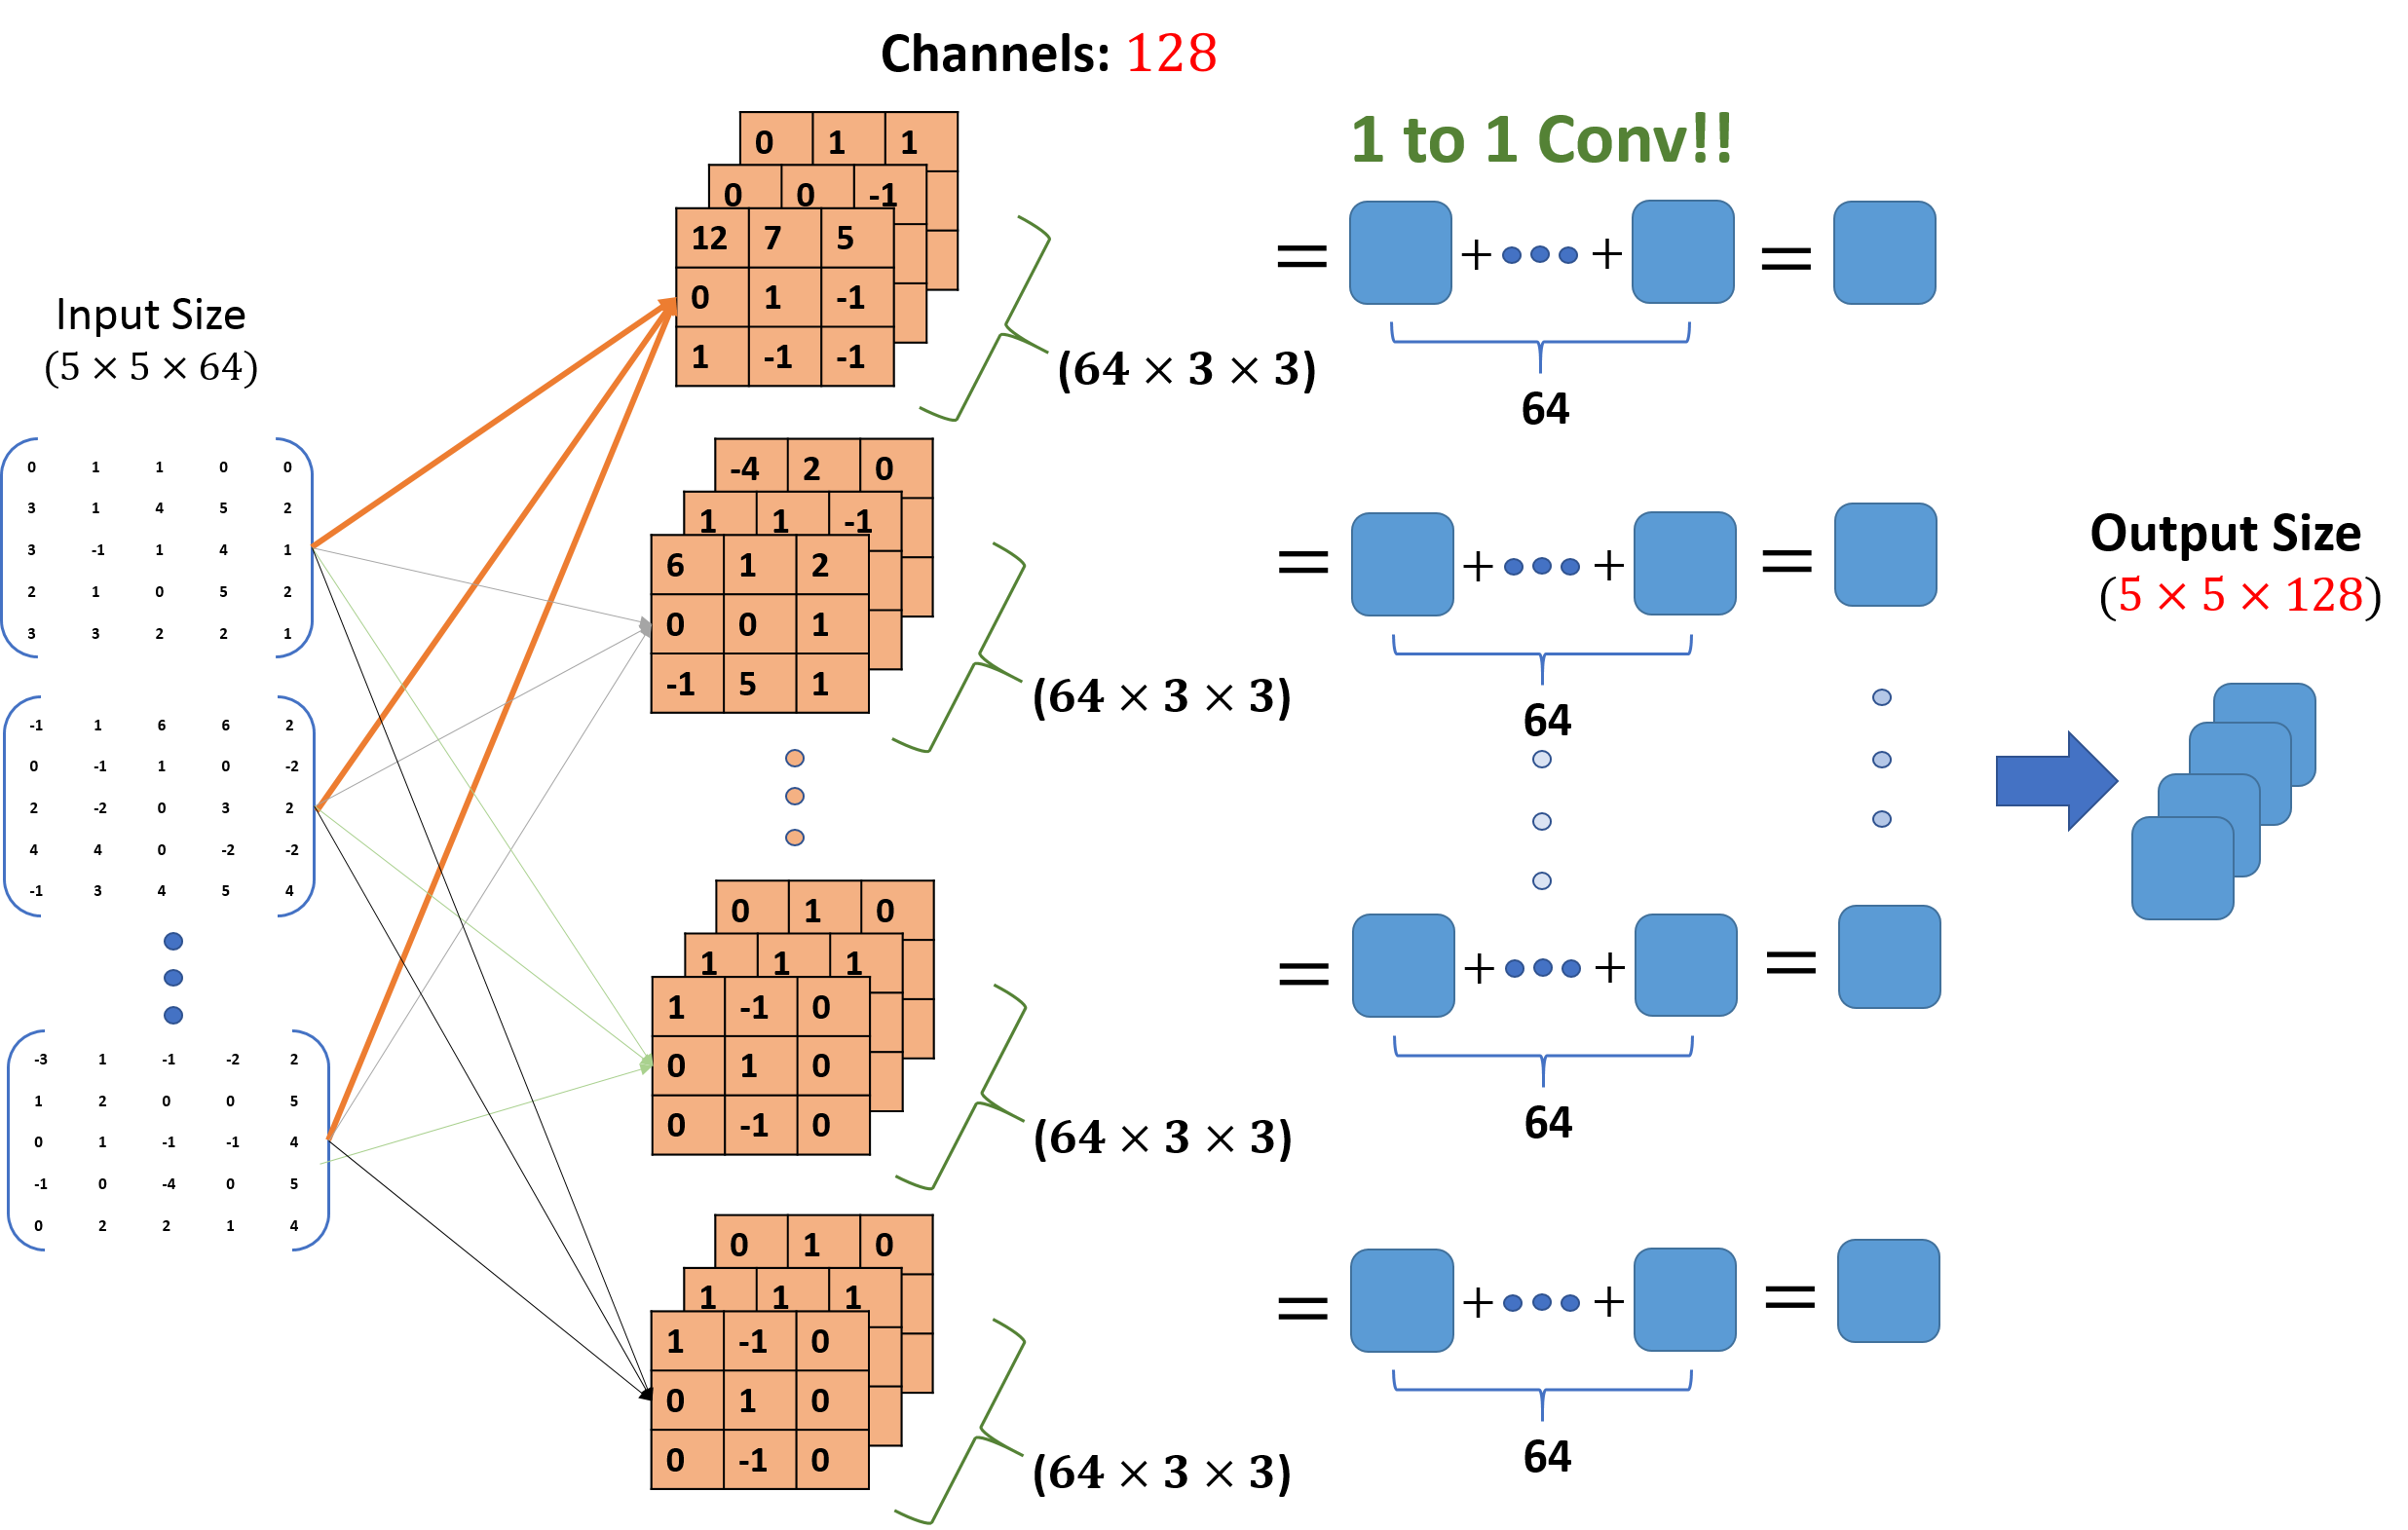
\includegraphics[width=1.0\textwidth]{convolution_2nd_layer2.png}
		}
	\caption{Each channel has 64 different $3\times 3$ filters. Each filter convolves with only \textit{one} channel of the input feature map!}
	\end{figure}
\end{frame}

\begin{frame}
\frametitle{A Short Break: A few questions ...}
Suppose we have $4 \times 512 \time 512 \times 1$ image as network input. That is, (batch size) 4 images where each of them is $512 \times 512 \times 1$ (gray images). Then,
\begin{itemize}
	\item how many parameters (numbers in filters) do we have so far for the first two layers?
	\pause
	\begin{itemize}
		\item $64\times 3 \times 3 + 128\times 64 \times 3 \times 3 = 576 + 73728 = 74,304$
	\end{itemize}
	\pause
	\item since both the batches, feature maps are stored in memory, how much memory do we need? (suppose padding $= 1$, stride $ = 1$)
		\begin{align*}
		&4 \times 512 \times 512 \times 1 + 4 \times 512 \times 512 \times 64 + 4 \times 512 \times 512 \times 128 \\
		&\approx 1M + 67M + 134M = 202M \\
		&= 202 M \times 4\text{ bytes} \approx 770 \text{MB} \quad \text(202M\times4/1024^2)
		\end{align*} 
	\textbf{Some background.} Almost all deep learning models are trained on GPUs. A typical GPU now has $6 \sim 8$ GB memory. Advance GPUs has $12$ GB memory (\eg \text{ } Nvidia GeForce GTX TITAN Z $\sim \$1.5K$ on amazon). 
\end{itemize}

\end{frame}
\begin{frame}
\frametitle{Batch Normalization (Conv + \textcolor{pink}{\textbf{BN}} + ReLU)}
In practice, to increase the training as well as testing speed, we usually feed \textbf{multiple} images to the network. The following figure shows a training batch of 4 images,
	\begin{figure}[H]
		\centerline{
			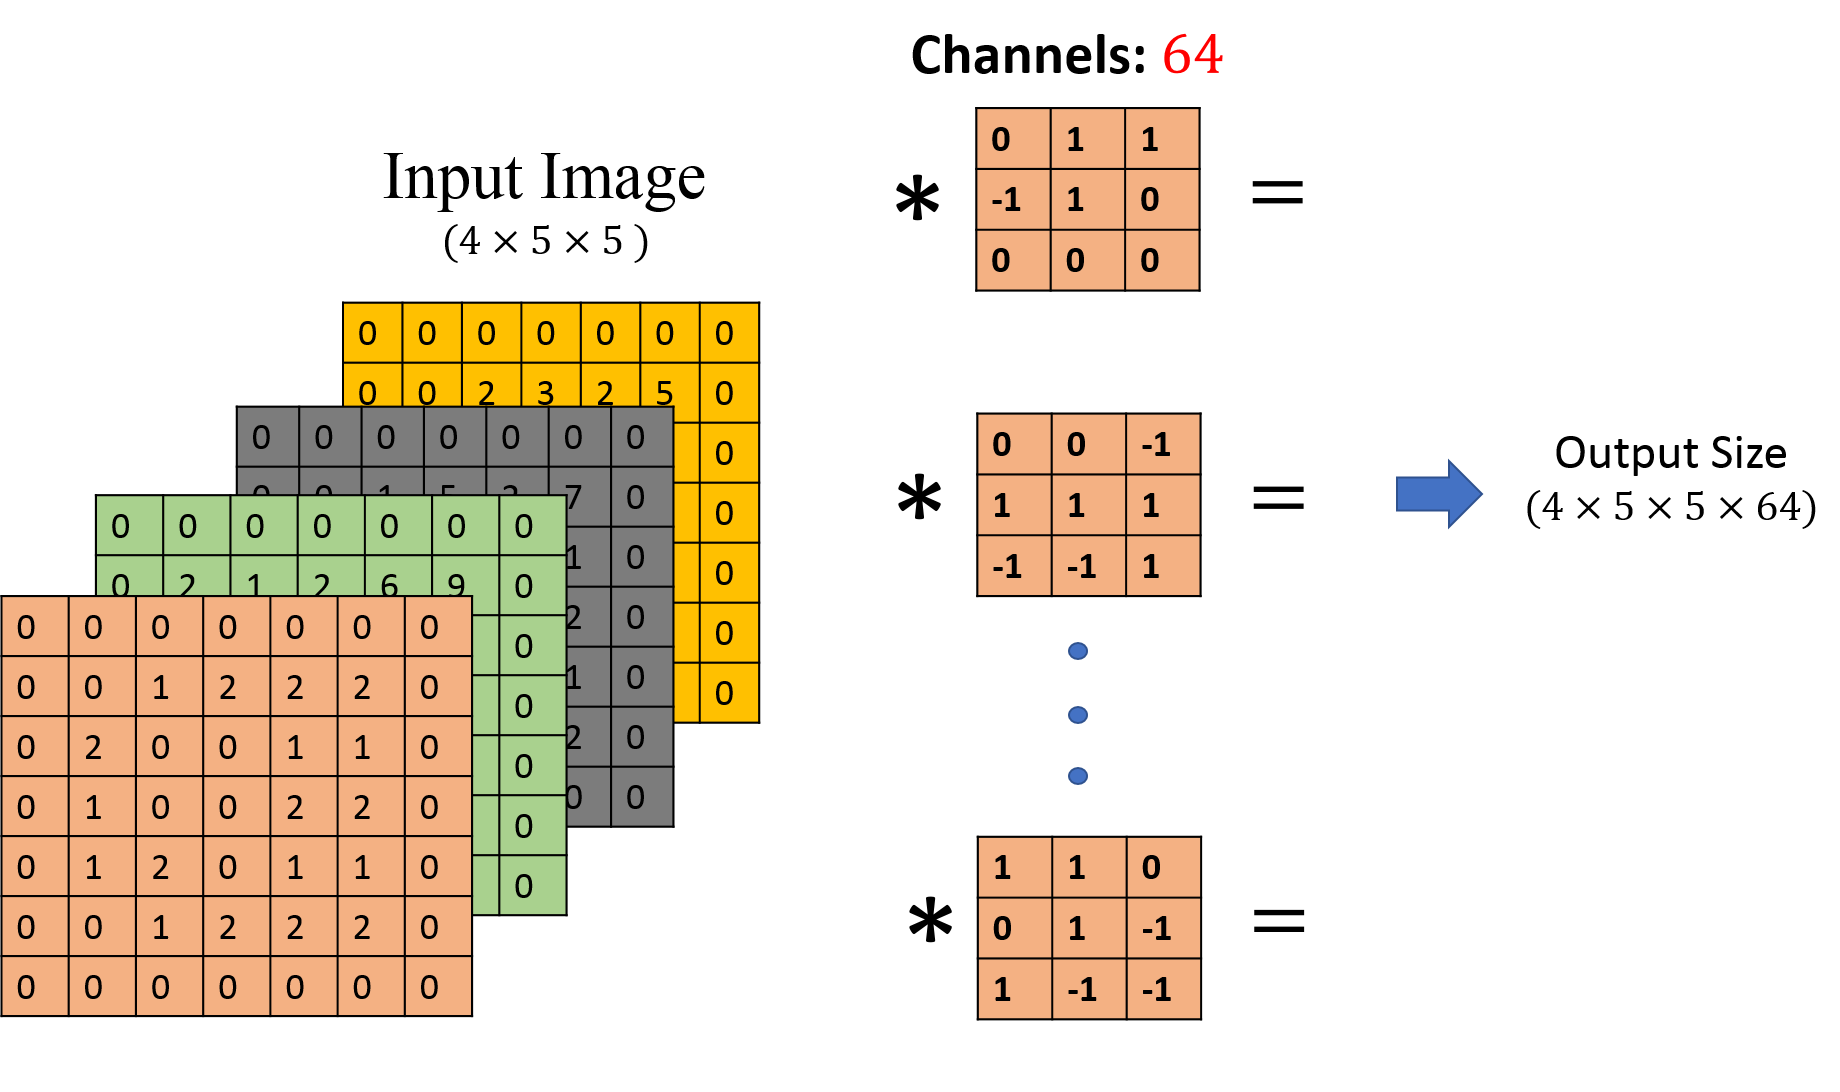
\includegraphics[width=0.9\textwidth]{batch.png}
		}
		\caption{Batch Size is 4. Each Image is independently processed.}
	\end{figure}
\end{frame}


\begin{frame}
	\frametitle{Batch Normalization \blfootnote{\textcolor{mycite2}{Sergey Ioffe, Christian Szegedy}.\textit{ Batch Normalization: Accelerating Deep Network Training by Reducing Internal Covariate Shift}, NIPs 2015.}: (Conv + \textcolor{pink}{\textbf{BN}} + ReLU)}
	For each \textbf{\textit{channel}}, normalize the layers. Mean bad variance are computed across all the values in each channel.
	\begin{figure}[H]
	\centerline{
		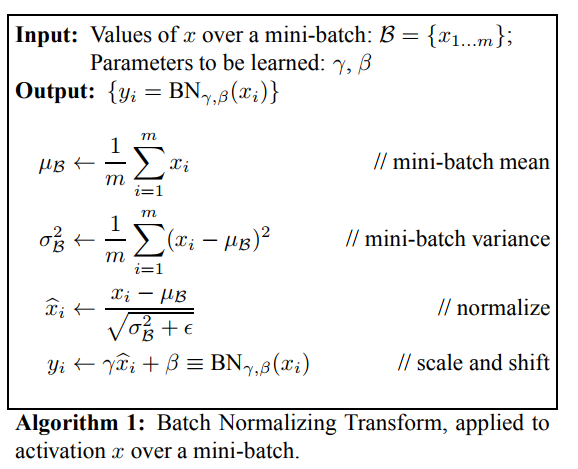
\includegraphics[width=0.6\textwidth]{BN.png}
	}
	\end{figure}	
\vskip -0.3in
	An effective way to resolve \textbf{\textit{vanishing gradient}} problem! 
\end{frame}

\begin{frame}
\frametitle{Nonlinear Activations: (Conv + BN + \textcolor{pink}{\textbf{ReLU}})}
Popular nonlinearities used through all \textbf{but} last layer:
\begin{itemize}
	\item ReLU: $\max (0, x)$.
	\item Leaky ReLU: $\max(0,x) + \gamma^2 \min(0,x)$
	\item Tanh: $\frac{\exp(x) -\exp(-x)}{\exp(x) + \exp(-x)}$
	\item Others \footnote{A good place to find all these is the document of deep learning software frameworks, eg. \url{http://pytorch.org/docs/master/nn.html}}: ELU, SELU, PRELU, Threshold \etc
\end{itemize}
	\begin{figure}
		\centering
		\subfloat[ReLU]{
			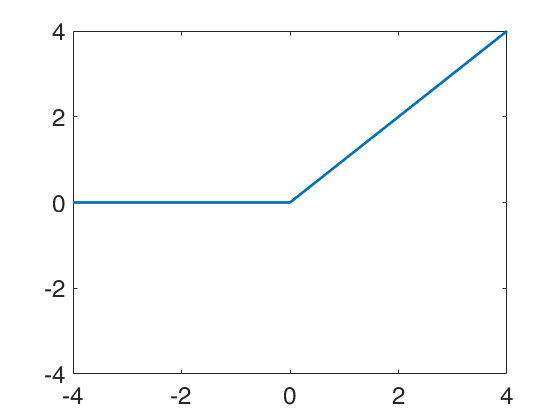
\includegraphics[width=0.33\textwidth]{relu.png}}
		\subfloat[Leaky ReLU]{
			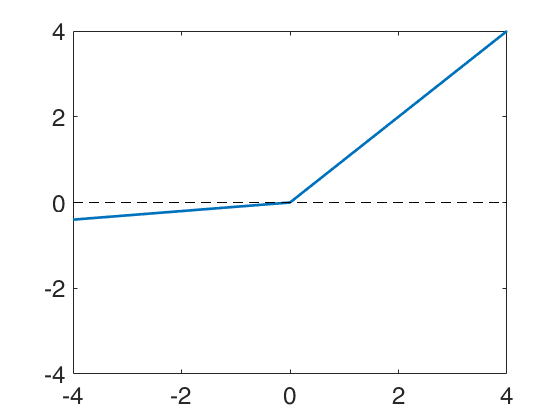
\includegraphics[width=0.33\textwidth]{lrelu.png}}
		\subfloat[Tanh]{
			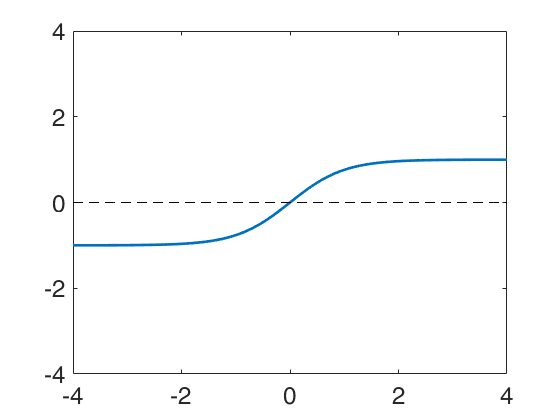
\includegraphics[width=0.33\textwidth]{tanh.png}}
	\end{figure}
\end{frame}

\begin{frame}
\frametitle{Pooling}
	\begin{figure}[H]
	\centerline{
		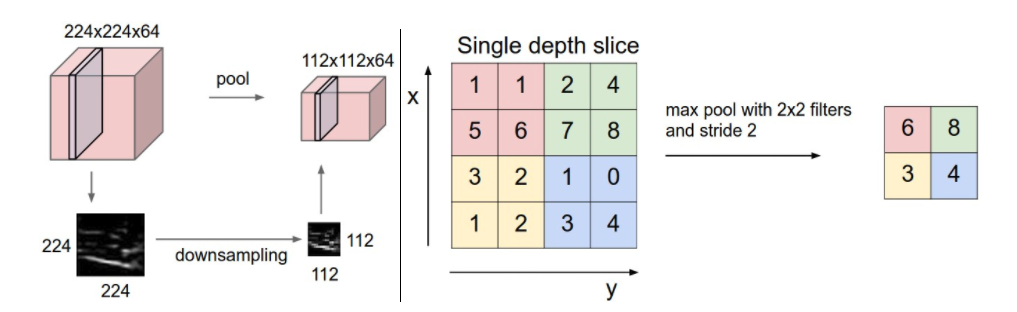
\includegraphics[width=1.0\textwidth]{pooling.png}
	}
	\caption{Illustration of \textit{Max Pooling}. Here batch size 1 is omitted. \footnote{Image courtesy of  CS231n: Convolutional Neural Networks for Visual Recognition.  Stanford.}}
	\end{figure}
	There is also average pooling which takes average rather than maximum.
\end{frame}

\begin{frame}
	\frametitle{Skip Connection}
	\begin{figure}[H]
	\centerline{
		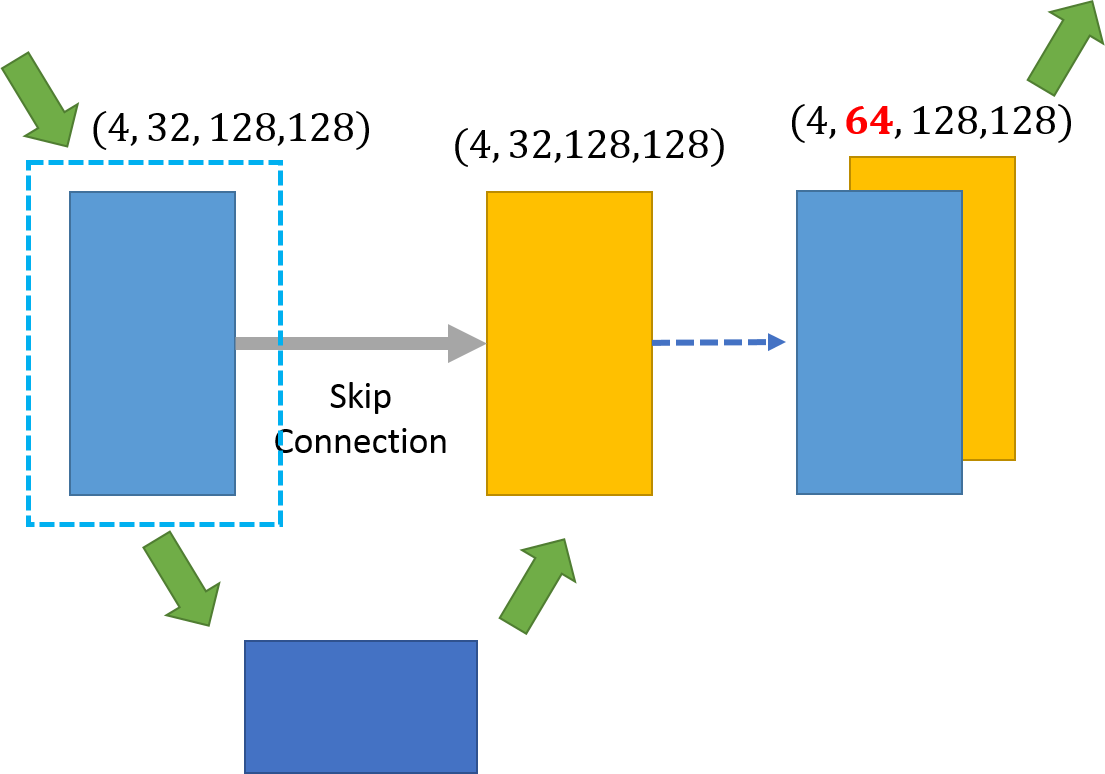
\includegraphics[width=0.6\textwidth]{skip.png}
	}
	\caption{Skip connection is simply concatenating two feature maps (along channel dimension). Central crop is performed is there is a miss-match of the dimension.}
	\end{figure}	
\vskip -0.2in 
	\textbf{Comment.} Adding skip connections can usually increase the performance (at least) in segmentation.
\end{frame}

\begin{frame}
\frametitle{Now We Know ($+-\times \div$) ...}
	\begin{figure}[H]
	\centerline{
		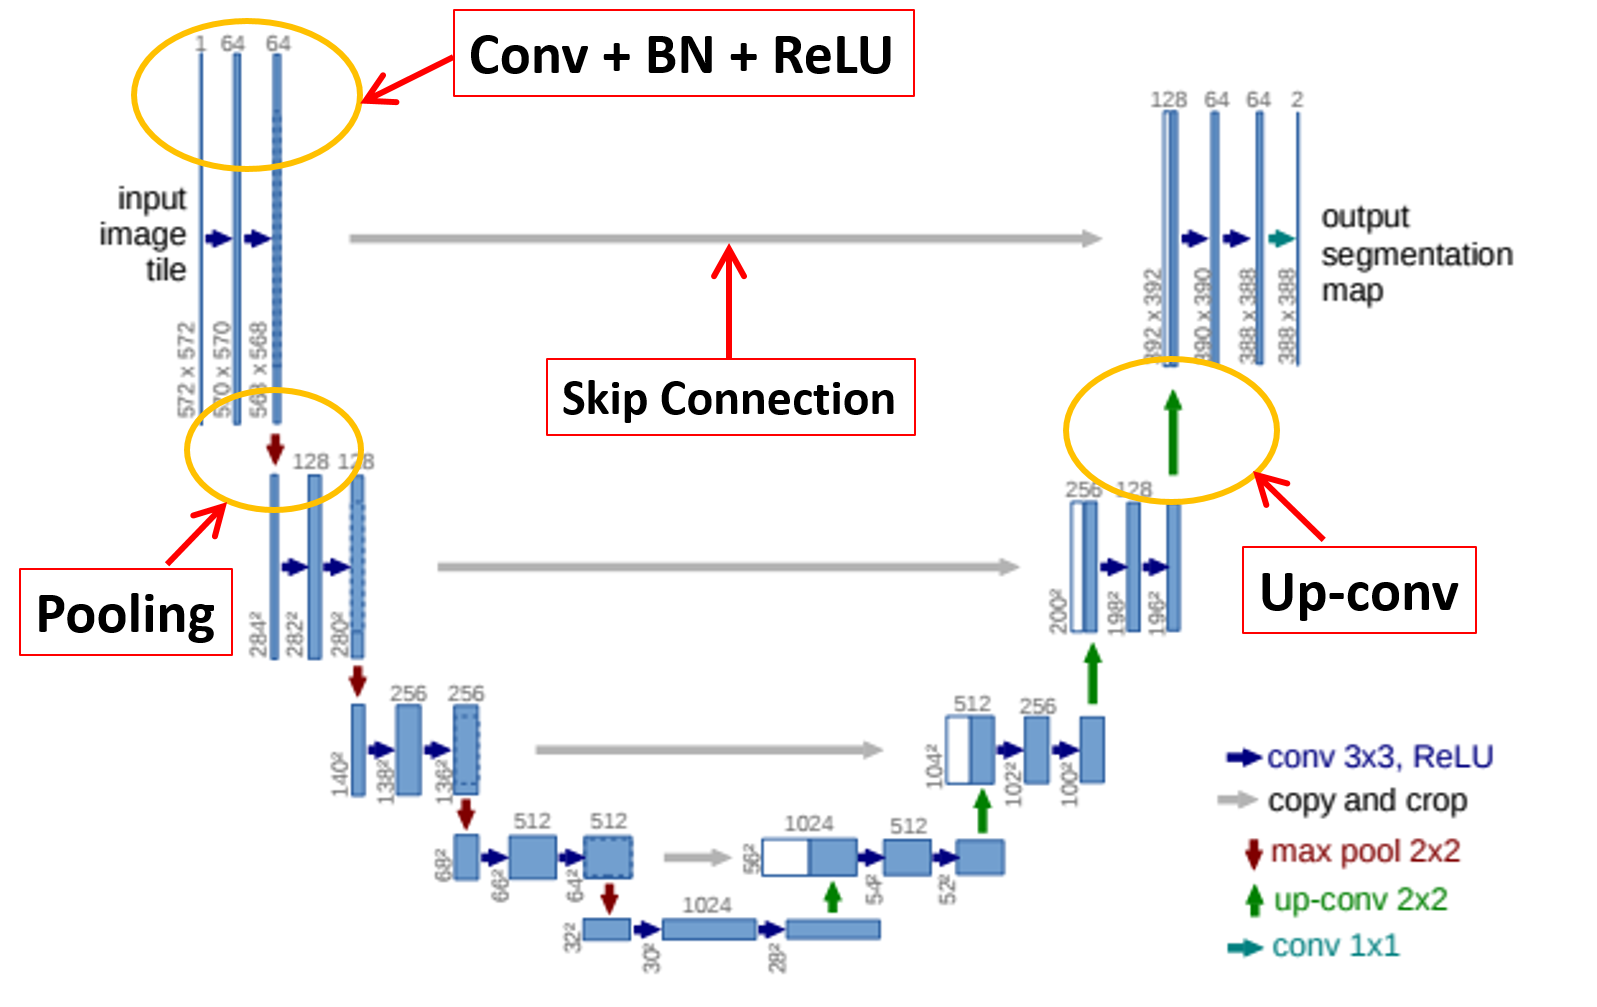
\includegraphics[width=0.8\textwidth]{unet_detailed.png}
	}
	\caption{Networks are just special ways to stack all these operations.}
\end{figure}
\end{frame}


\subsection{Optimization Problems in CNNs}
\begin{frame}
\frametitle{Function Representation}
	\begin{figure}[H]
	\centerline{
		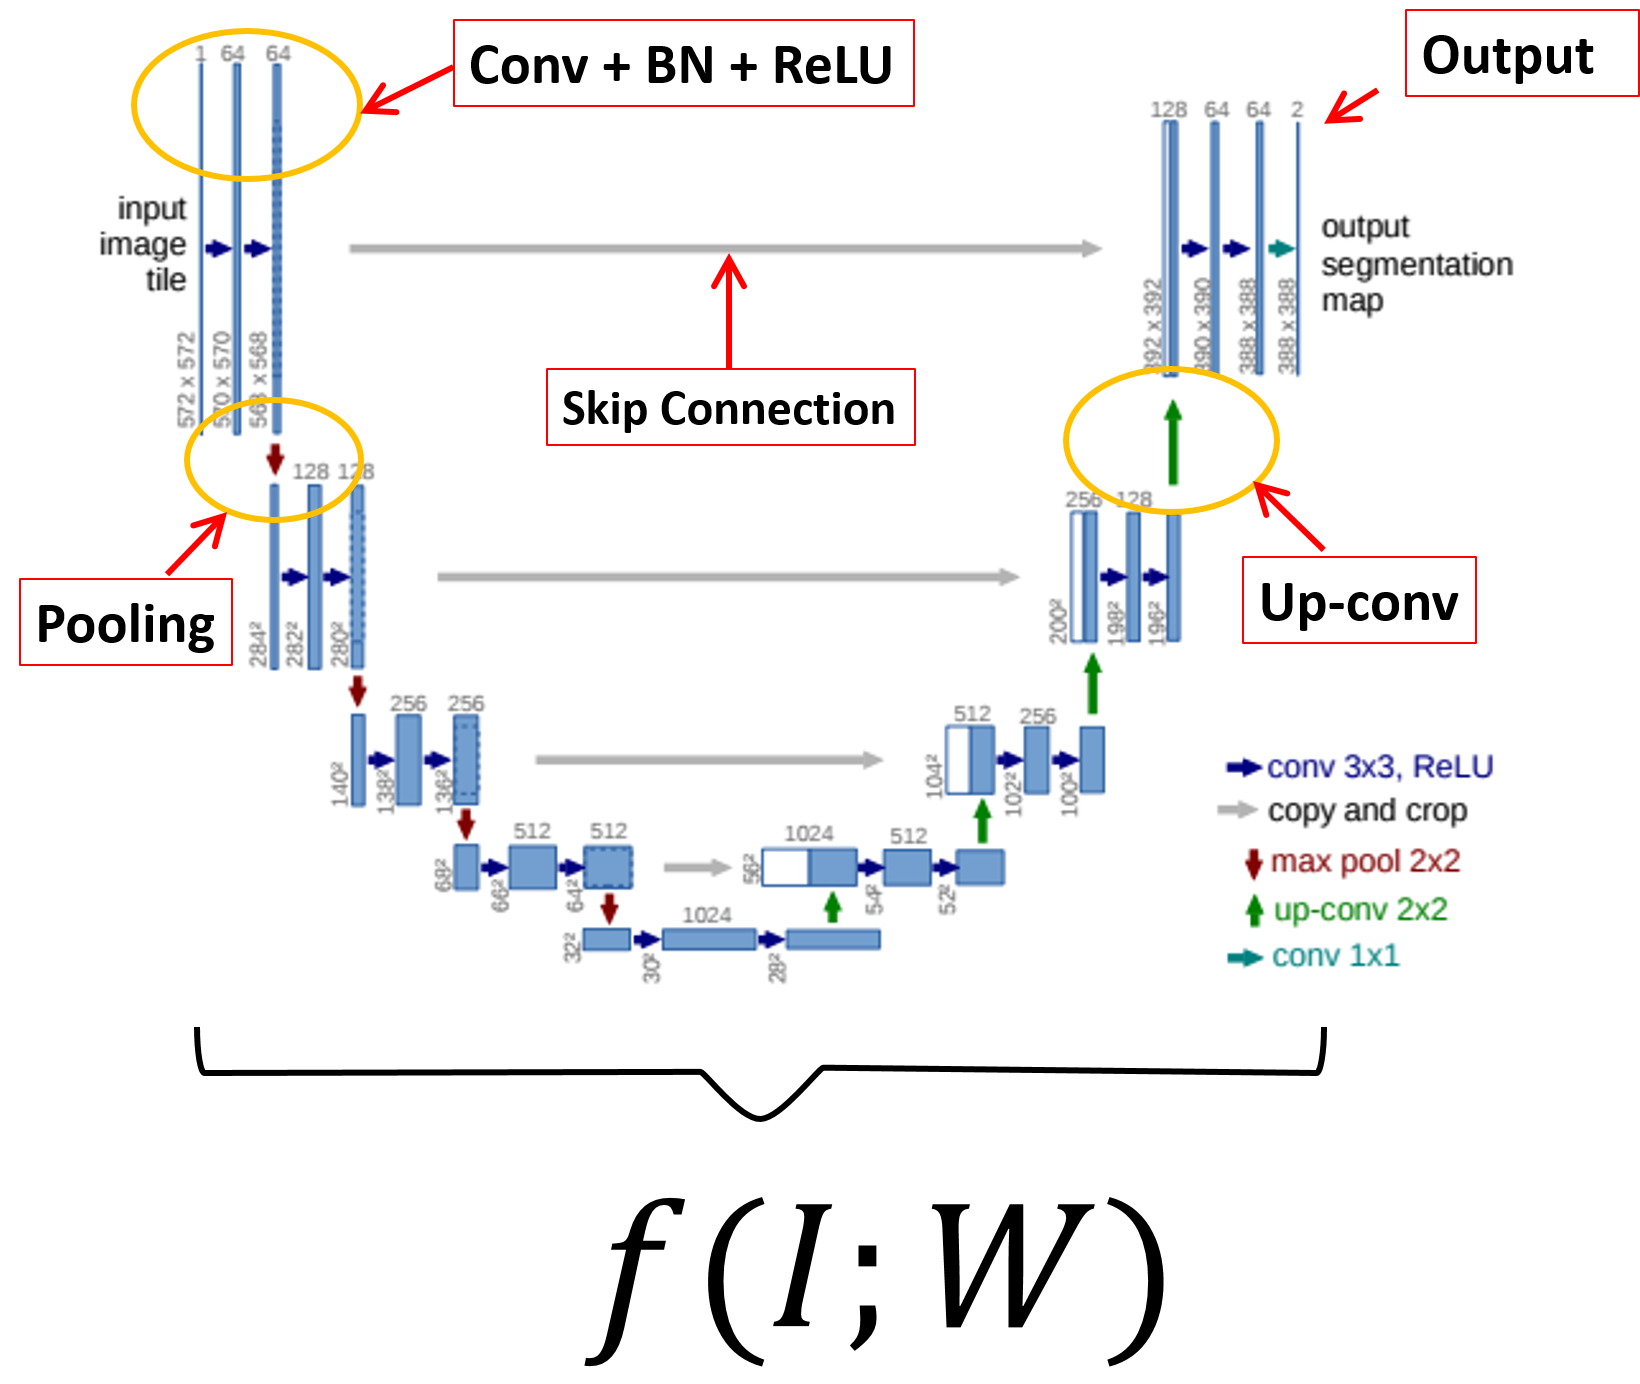
\includegraphics[width=0.6\textwidth]{optimization_fx.png}
	}
	\caption{The entire network is just another representation of $f(I; W)$, where $I$ is input image(s), $W$ are the parameters in the network.}
	\end{figure}
\end{frame}

\begin{frame}
\frametitle{Optimization Problem}
In training state, we are given ground truth images and its labels for recognition/classification, or masks for segmentation, high-resolution image for super-resolution, clear image for de-noising \etc. 
\vskip 0.2in
Let $I$ be the truth images and $g$ be their labels, the optimization problem is 
\[
\min_W \quad Loss\{ f(I; W) - g\}
\] 
Popular losses,
\begin{itemize}
	\item \textbf{$l_2$ distance}: image denoising, super-resolution, recognition.
	\item \textbf{Entropy}: binary/categorical cross-entropy, KL-divergence for segmentation.
	\item Many other \textbf{customized losses}, \eg \text{ } $l_1$ for GAN, smoothed dice loss for segmentation.
\end{itemize}
\end{frame}

\begin{frame}
\frametitle{Loss Function Example: Cross Entropy}
Suppose we are doing a single object segmentation, \eg\ lung. The last convolutional channel will have 2 channels corresponding foreground and background. 
	\begin{figure}[H]
	\centerline{
		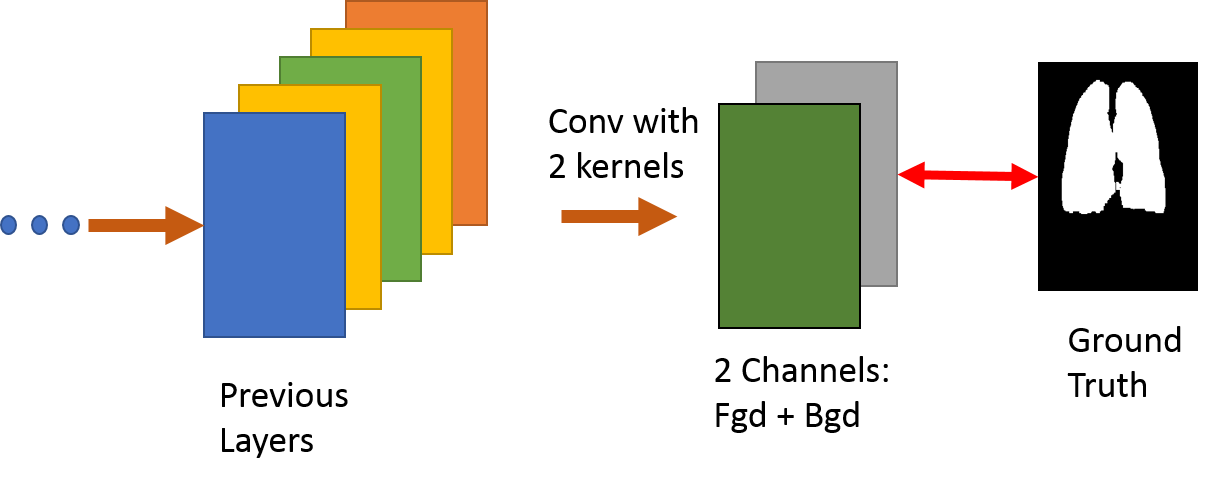
\includegraphics[width=0.8\textwidth]{last_layer.png}
	}
	\end{figure}
Softmax + Cross-entropy
\end{frame}
\section{Optimization}
\begin{frame}
	\frametitle{Overview}
%		\begin{figure}[H]
%			\centerline{
%				\includegraphics[width=0.7\textwidth]{bigdata}
%			}
%			\caption{Big data is too big, only few are important.}
%		\end{figure}
%	\vskip -0.1in
%	Mathematics of sparse modeling, 
%	\begin{align*}
%	&\min \text{ } Loss(x)  \\
%	&\text{s.t. } g(x) \text{ is sparse}.
%	\end{align*}
\end{frame}

\section{Networks Variants}
\begin{frame}
\frametitle{Networks}
	\begin{figure}[H]
	\centerline{
		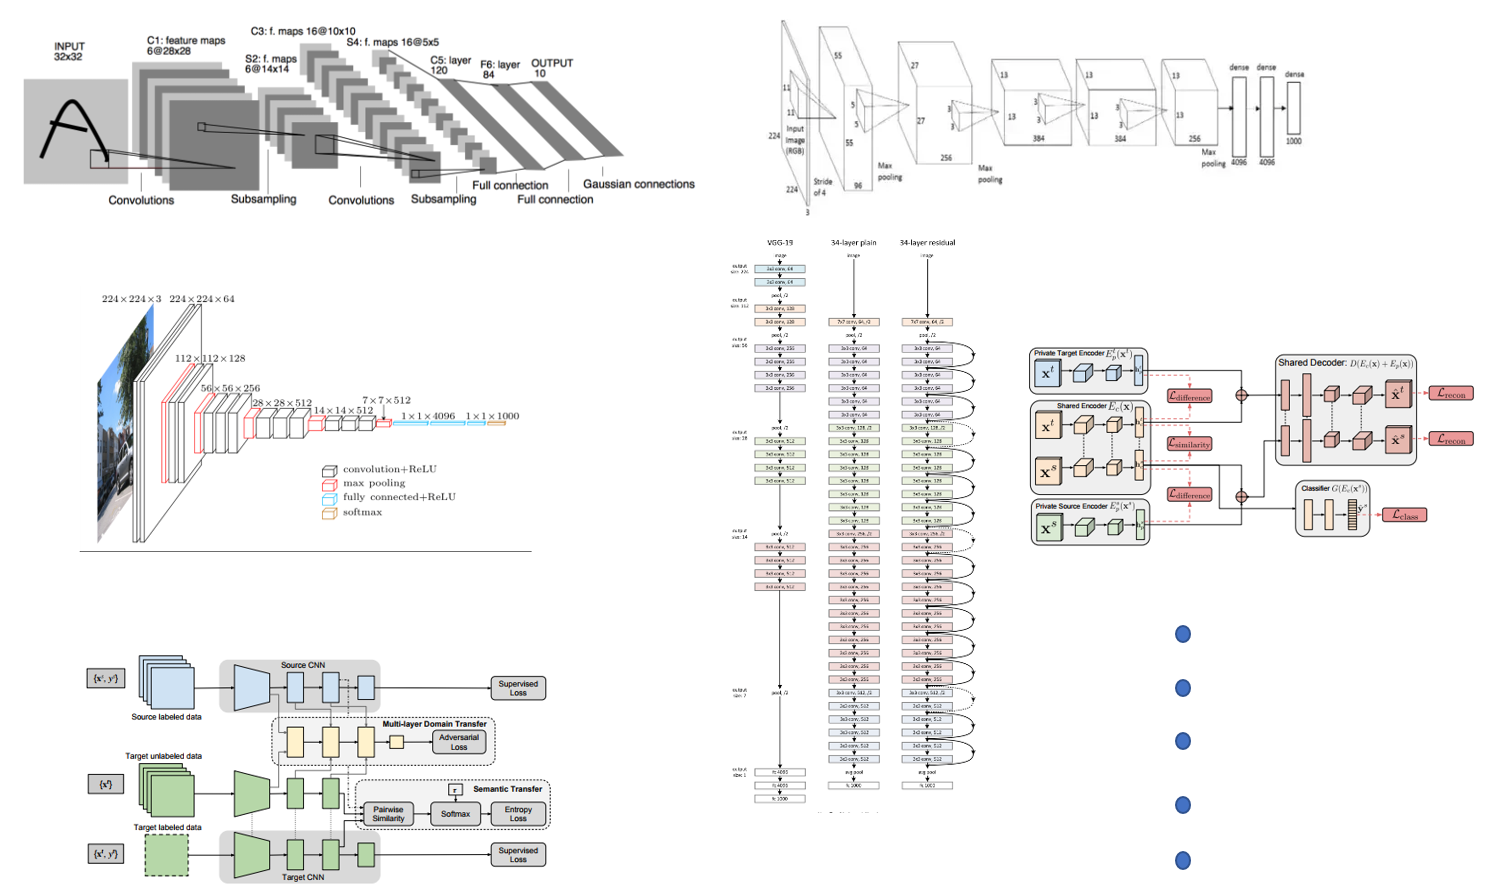
\includegraphics[width=0.8\textwidth]{networks.png}
	}
	\caption{Networks are just special ways to stack all these operations.}
\end{figure}
\end{frame}

\section{Coding}
\begin{frame}
\frametitle{Frameworks}
\end{frame}

\begin{frame}
	\begin{center}
		{\textcolor[rgb]{1 0 0}{\Huge\textsc{Thank you!}}}\bigskip
	\end{center}
\end{frame}




\end{document}
